\documentclass{beamer}
%
% Choose how your presentation looks.
%
% For more themes, color themes and font themes, see:
% http://deic.uab.es/~iblanes/beamer_gallery/index_by_theme.html
%
\mode<presentation>
{
  \usetheme{default}      % or try Darmstadt, Madrid, Warsaw, ...
  \usecolortheme{seahorse} % or try albatross, beaver, crane, ...
  \usefonttheme{default}  % or try serif, structurebold, ...
  \setbeamertemplate{navigation symbols}{}
  \setbeamertemplate{caption}[numbered]
} 

\usepackage[english]{babel}
\usepackage[utf8]{inputenc}
\usepackage[T1]{fontenc}
\usepackage{wrapfig}
\usepackage{hyperref}
\usepackage{amsmath}


\title[cs370 Final]{Kitty's Calculations on a Tree}
\author{Eric Altenburg, Hamzah Nizami, and Connie Xu}
\institute{I pledge my honor that I have abided by the Stevens Honor System.}
\date

\begin{document}

\begin{frame}
  \titlepage
\end{frame}

\begin{frame}{Outline}
  \tableofcontents
\end{frame}

\section{Introduction}
\begin{frame}{What is Kitty's Calculations on a Tree?}
Link to problem: \href{https://www.hackerrank.com/challenges/kittys-calculations-on-a-tree/problem}{\color{blue}here}
\begin{itemize}
  \item You are given a tree and a set of subsets.
  \item The goal of this is to calculate the below expression on each of the sets.
\end{itemize}
\begin{align*}
(\sum_{u,v} u * v * dist(u,v)) \mod (10^9 + 7)
\end{align*}
\end{frame}

\begin{frame}{Kitty's Calculations on a Tree Continued}
\begin{figure}
\begin{subfigure}{ }
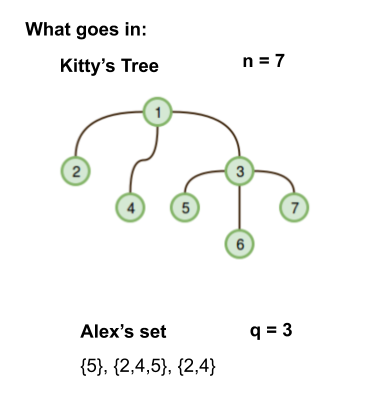
\includegraphics[scale=.3]{Kittycalc.png} 
\end{subfigure}
\begin{subfigure}{ }
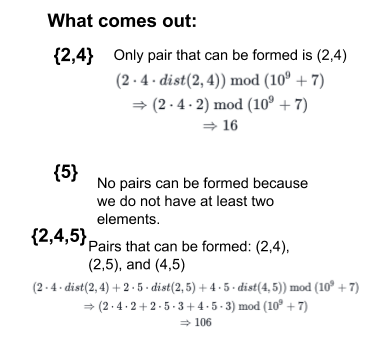
\includegraphics[scale=.3]{Kittycalcbottom.png}
\end{subfigure}
\caption{Shows an example input and expected output}
\label{fig:image2}
\end{figure}
\end{frame}

\section{Problem Constraints}

\begin{frame}{Constraints of the problem}
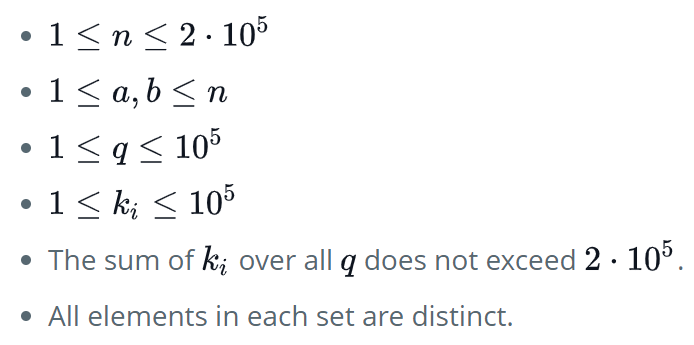
\includegraphics[scale=.7]{constraintskitty.PNG}
\vspace{.5cm}
\\n is the number of nodes on a tree, a,b are the subset pairs in the tree, q is the number of sets, and k is the number of distinct nodes
\end{frame}

\section{Test Cases}
\begin{frame}{Test Cases and Descriptions}
The first test case is shown in Figure 1 in our presentation. This test case is a simple test case to ensure that our code runs properly.
\begin{itemize}
    \item The first number on line 1 denotes how many nodes are in the tree. 
    \item The second number on line 1 denotes the number of sets. 
    \item The following n-1 lines will show the pair of integers that are connected in the tree. 
    \item Then, the subsequent lines will first denote the number of elements in the set, and then the next line will be which numbers are in each set.
\end{itemize}
\end{frame}

\begin{frame}{Test Cases and Descriptions}
The syntax for the input is the following:
\\
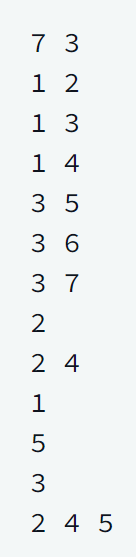
\includegraphics[scale=.7]{inputkitty01.PNG} 
\end{frame}

\begin{frame}{Test Cases and Descriptions}
The output of the above test case should yield for each set, the summation of each. Hence, this should return 16, 0, and 106, respectively (as the first set {2,4}, the second set is {5} and the third set is {2,4,5}).
\\To find all of the test cases, just click \href{https://github.com/conniexu444/kittyscalculationstestcases}{\color{blue}here}.
\end{frame}

\section{Tracing Time}
\begin{frame}{Time to Trace!}
Now, we shall trace!
\end{frame}

\section{Failed Attempts}
\begin{frame}{Failed Attempts}
The different approaches we took before we arrived at our current solution are the following:
\begin{itemize}
    \item Brute Force-ish
    \begin{itemize}
        \item We attempted to implement a tree and we traversed it with the distance and did what the problem described to do, but it was too slow. 
    \end{itemize}
    \item Floyd's Algorithm
    \begin{itemize}
        \item This did not work because we quickly realized that this would likely exceed the time limit. This algorithm also proved to be tough to implement with this problem so we moved on and tried a different approach.
    \end{itemize}
    \item Intermediate vertices
    \begin{itemize}
        \item Looking at the intermediate vertices proved futile as we attempted this problem. It did not provide helpful information on its own. 
    \end{itemize}
    \item Depth first search
    \begin{itemize}
        \item DFS on its own was not the solution. If the tree was too deep, this algorithm would have exceeded the time limit on its own. 
    \end{itemize}
\end{itemize}
\end{frame}

\begin{frame}{Failed Attempts}
\begin{itemize}
    \item Formula manipulation
    \begin{itemize}
        \item We thought messing with the formula may be effective as with previous homework from 370, but this information alone was not quite helpful. 
    \end{itemize}
    \item Lowest Common Ancestor
    \begin{itemize}
        \item Alone, this did not work. 
    \end{itemize}
\end{itemize}
With most of the attempts to find a solution, we found ourselves failing due to time constraints, space constraints, or incorrect implementation.
\\Ultimately, we found that a combination of lowest common ancestor and formula manipulation was the way to go and this is what we ended up implementing. There was a lot of tracing that went into this. 
\end{frame}



\end{document}
